\subsection{Linear Separability}

As stated before, a perecptron is a binary classifier. A fairly obvious application of the concept is for classification. There are several instances where classification is necessary. \\
		
		For this report, we have chosen a rudimentary example of a classification task: \textbf{Linear separability}. Consider a set of blue points and a set of red points on a two-dimensional plane. The two sets are linearly separable if there exists a line on the plane such that all of the blue points lie on one side of the plane and all of the red points lie on the other side. \\

\begin{center}
	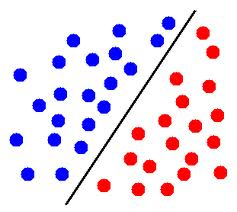
\includegraphics[scale=0.5]{ls}
\end{center}

Shown above is an instance of two-dimensional linear separation. This idea is immediately generalized to n-dimensional Euclidean spaces if the line is replaced by a hyperplane.

\subsection{How is the Perceptron useful here?}
Recall that a Perceptron accepts a set of inputs and produces an output of either 0 or 1. We can pass in the coordinates of each point along with the bias (which we will explain later) and the expected output. This will be a $4x1$ column vector. We will call our input vector $x$. \\

	\begin{center}
		$x = 
		\begin{bmatrix}
			b \\
			i1 \\
			i2 \\
			y
		\end{bmatrix}
		$
	\end{center}

where $b$ is the bias, $i1$ is the x-coordinate of the point, $i2$ the y-coordinate, and $y$ is the expected output (0 or 1). \\

\subsection{Implementing the Perceptron}
We decided to use Python to implement the algorithm. We generated 10 random two-dimensional points such that they are linearly separable. \\

	\begin{center}
		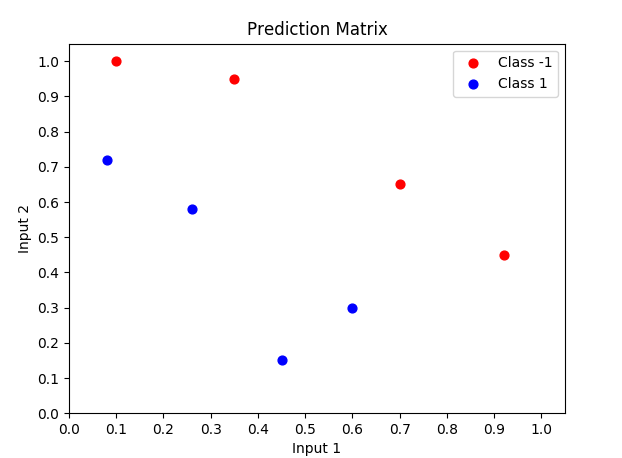
\includegraphics[scale=0.5]{pts}
	\end{center}
	
Shown above is are the 10 points plotted. Notice how there is a line (with slope $\approx$ -1) that can separate the two sets. The points above the line will be Class -1 and have a color of Red, while the points below the line will be Class 1 and have a color of Blue. \\

We will first implement a function $predict()$ that will return the appropriate class for a specified set of inputs and their corresponding weights. \\


	\begin{lstlisting}[language=Python, frame=single]
# Returns 1 if the weighted input sum is greater 
# than a threshold.
def predict(inputs, weights):
    activation_threshold = 0.0

    # Obtaining the weighted sum of the inputs.
    for i, w in zip(inputs, weights):
        activation_threshold += w * i

    return 1.0 if activation_threshold >= 0.0 else 0.0
	\end{lstlisting}
	
	\begin{enumerate}
		\item Initialize the $activation\_threshold$ to $0.0$. Any value above it will return 1, and any value below will return 0.
		
		\item Iterate through the inputs and their corresponding weights and calculate the weighted sum. The function \textbf{zip} lets us iterate through both the inputs and the weights parallely. We store the sum in the $activation\_threshold$ variable.
		
		\item Return the appropriate class depending on the value of the weighted sum.
	\end{enumerate}

Next, we implement a function $accuracy()$ that will calculate the percentage accuracy of the classifier during each iteration. \\ 

	\begin{lstlisting}[language=Python, frame=single]
# Returns the percentage accuracy of the classifier.
def accuracy(matrix, weights):
    num_correct = 0.0
    preds = []

    for i in range(len(matrix)):
        pred = predict(matrix[i][:-1], weights)
        preds.append(pred)

        if pred == matrix[i][-1]:
            num_correct += 1.0

    print("Predictions:", preds)

    return num_correct / float(len(matrix))
	\end{lstlisting}
	
	\begin{enumerate}
		\item Initialize $num\_correct$ to $0.0$ (number of correct predictions) and $preds$ to an empty array (we will store multiple predictions in this array). 
		
		\item We iterate through the $matrix$. $matrix$ is a two-dimensional array, i.e., a collection of data vectors. The function \textbf{len} allows us to calculate the number of data vectors in $matrix$. 
		
		\item We add the predicted class of each data vector to the $preds$ array. Note that each prediction is itself an array, so this makes $preds$ a two-dimensional array.
		
		\item If the predicted class matches the expected class, then we increment $num_correct$. 
		
		\item We print out the list of predictions and return the ercentage accuracy of the predictions. The \textbf{float} function helps us prevent truncation (rounding down) of the answer to give us a better answer.
	\end{enumerate}
	
	Finally, we implement our backpropogation algorithm, where we update the weights after each iteration to improve the predictions made by the perceptron.

	\begin{lstlisting}[language=Python, frame=single]
# Backpropogation algorithm
def train_weights(matrix, weights, n_iteration=10, 
l_rate=1.00, do_plot=False, stop_early=True, 
verbose=True):

    for epoch in range(n_iteration):
        current_accuracy = accuracy(matrix, weights)
        print("\nEpoch %d \nWeights: " %epoch, weights)
        print("Accuracy: ", current_accuracy)

        # If the maximum accuracy is reached
        if current_accuracy == 1.0 and stop_early:
            break

        if do_plot:
            plot(matrix, weights, title="Epoch %d" 
            %epoch)

        for i in range(len(matrix)):

            # Current prediction
            prediction = predict(matrix[i][:-1], 
            weights)

            # Error in prediction
            error = matrix[i][-1] - prediction

            # Updating the weights
            for j in range(len(weights)):
                if verbose:
                    sys.stdout
                    .write("\tWeight[%d]: %0.5f --> "
                    %(j, weights[j]))

                # Updating the weights.
                weights[j] += 
                (l_rate * error * matrix[i][j])

                if verbose:
                    sys.stdout
                    .write("%0.5f\n"
                    %(weights[j]))
    
    # Plotting the final matrix.
    plot(matrix, weights, title="Final epoch")
    return weights
	\end{lstlisting}
	
	\begin{enumerate}
		\item An epoch is a forward and backward pass when it comes to training. The number of iterations is the sum of the forward and backward passes. We thus have $\frac{n_iteration }{2}$ number of iterations in this function. We save the current accuracy into $current\_accuracy$. 
		
		\item Should our algorithm ever reach maximum accuracy, the \textbf{break} statement allows us to terminate the training process immediately. 
		
		\item Should we ever need to see the predictions visually each time ($do\_plot$ will have a value of \textbf{True} in this case), we plot the data and the line to separate them. 
		
		\item We then iterate through the $matrix$ (which is again a two-dimensional array) and save the error of our prediction into $error$.
		
		\item Using the error in our prediction, we then iterate through $weights$ (this is an array of values that we change each time the $train\_weights()$ function is called. In each iteration, we update $weights[j]$ (which is the jth value in the $weights$ array) using the following formula \\
		\begin{center}
			$w_j = w_j + (l * e_i * M_{i, j})$
		\end{center}
		
		where $w_j$ is the $j^{th}$ value in the $weights$ array, $l$ is the learning rate (a measure of how fast the perceptron should learn that was chosen arbitrarily), $e_i$ is the error in prediction for the $i^{th}$ data vector in $matrix$, and $M_{i, j}$ is the $j^th$ value in the $i^{th}$ data vector (the corresponding input to the weight).
		
		\item The $verbose$ variable is a boolean value. If it is \textbf{True}, we print out the value of the weights before and after they are updated. 
		
		\item Regardless of whether we plot the line and data points during each iteration, we plot the points and the line after the iteration terminates. 
		
		\item Finally, we return the updated $weights$.
	\end{enumerate}
	
\subsection{The Results}
Shown below are the plots from each epoch. Note that we start the number at $0$. We have $\frac{10}{2} = 5$ epochs.

	\begin{enumerate}
		\item Epoch 0: Since we set the $weights$ vector arbitrarily, our line of separation is highly inaccurate.
		
		\item Epoch 1: Since we updated the weights, the perceptron 'realizes' that the line of separation was inaccurate due to the high error rate it would have received. Hence, we do not see much of a line in this epoch.
		
		\item Epoch 2: 
	\end{enumerate}

\begin{center}
	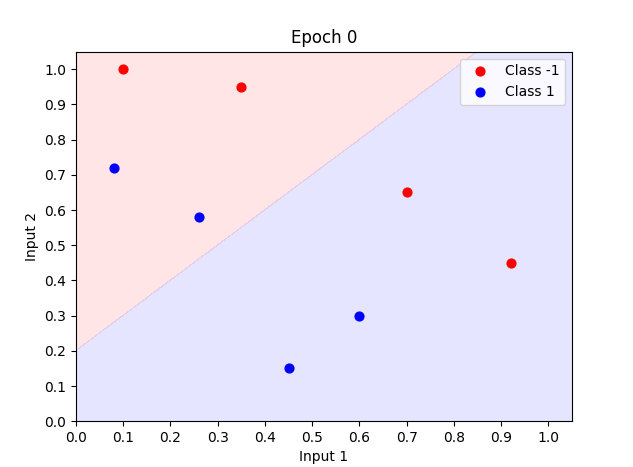
\includegraphics[scale=0.4]{e0}
	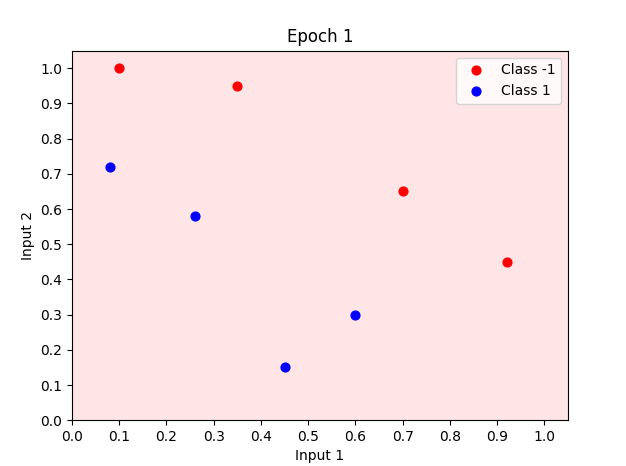
\includegraphics[scale=0.4]{e1}
	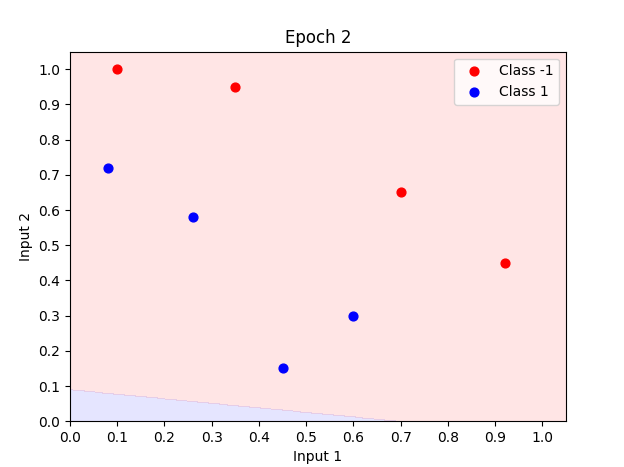
\includegraphics[scale=0.4]{e2}
	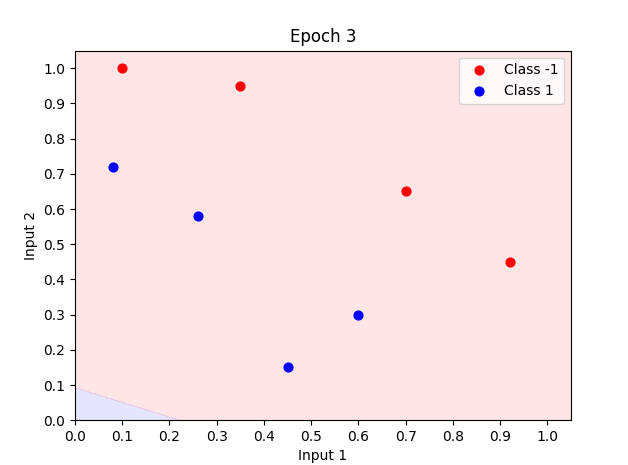
\includegraphics[scale=0.4]{e3}
	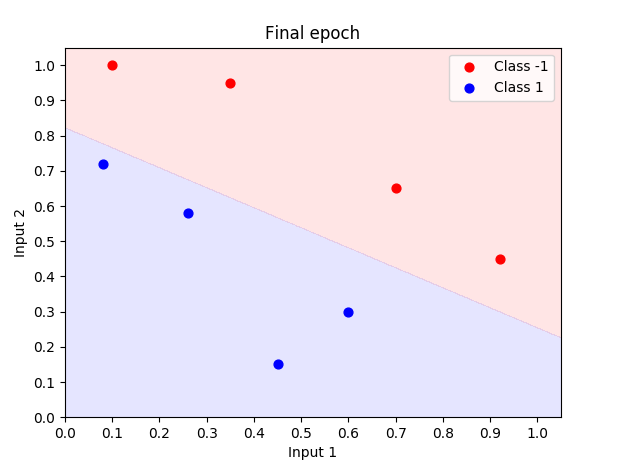
\includegraphics[scale=0.4]{e10}
\end{center}